\documentclass[12pt]{article}
\usepackage{blindtext}
\usepackage{graphicx}

\graphicspath{{./images/}}

\title{Finding the most efficient braking position for any bike\\
	\large International Baccalaureate Extended Essay}
\author{Igor Krzywda}

\begin{document}
\maketitle

\section{Introduction}
\subsection{Context}
Braking is the most important safety feature on a bicycle, however when misused braking can be the cause of the
most severe crashes one can have on a bicycle. Many of such crashes are caused by the lack of understanding of
mechanics of braking a bicycle. There are countless tutorials as how to brake properly on a bicycle, but most of
them are based on empirical experience of more proffesional riders. Such advice falls in line with physical 
analysis, but is mostly biased by many factors spanning from the type of cycling the tutorial is based on to 
the attitude towards crashing of the presenter. There is clearly a void in giving an objective advice on safety 
on a bicycle that can be a base to domain-specific guides.

\subsection{Scope of research}
This essay will be exploring the placement of centre of mass for maximum braking while maintaining safety. 
The analysis will be split into two parts-a theoretical one involving building an universal model for finding 
best braking setup and a practical one, which will serve as a validation of the theoretical model using sensor
data.

\subsection{The goal of the research}
The goal of the research is to create an universal model for finding the best braking position in terms of
centre of mass on any bicycle. Such model will serve as a basis for explaining why it is important to find 
a bike fitting its rider and giving the reader an idea of where the limits of his equipment are without 
finding about it by crashing.

\section{Theoretical analysis of braking a bicycle}
\subsection{Rules and assumptions for the analysis}
Assumptions about bicycle and rider:
\begin{itemize}
\item{the rider is a stiff body}
\item{there is no dissipation of force}
\end{itemize}
Safe braking in the analysis is defined by two factors:
\begin{itemize}
\item{rear wheel makes contact with the surface at all times}
\item{no wheel is skidding while braking}
\end{itemize}
Neglected factors\footnote[1]{these factors play more significant role in reality than they do in theoretical
considerations}:
\begin{itemize}
\item{decrease in braking power due to heat and brake pad residue}
\item{dynamic change in frame geometry due to amortisation and tire compression}
\item{air drag}
\item{rolling resistance}
\end{itemize}
\newpage
\subsection{Forces acting on a bicycle when stationary}
When stationary, the only force acting on the bike is weight of the rider which gets split between bike's axles.
The proportion of force acting on front axle versus rear axle is dependent on the position of the centre of mass
of both bike and rider. \\
Force excerted on either axle is calculated from torque applied on the rear axle: \\
$F = \frac{\tau}{r}$\\
$F_f = \frac{d \cdot mg}{l}$\\
$F_r = mg - F_f$
\begin{figure}[h]
\centering
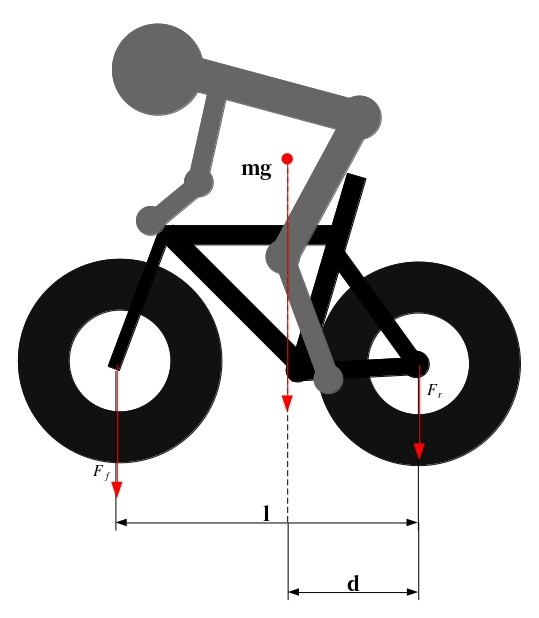
\includegraphics[width = 0.65 \linewidth]{static_with_forces_bike}
\caption{bicycle and rider diagram}
\end{figure}
\begin{figure}[h]
\centering
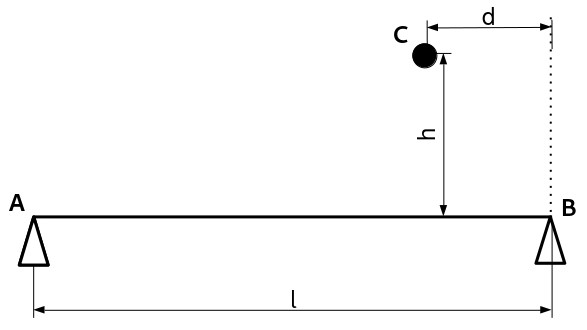
\includegraphics[width = 0.45 \linewidth]{bike_static_model_simplified}
\caption{simplified diagram of rider and bicycle}
\end{figure}

\subsection{Forces acting on a bicycle when braking}
\end{document}
